\documentclass{standalone}
\usepackage[utf8]{inputenc}
\usepackage{tikz}
\usetikzlibrary{arrows, positioning, fit, backgrounds, calc}
\usepackage{amsmath, amssymb}

\begin{document}
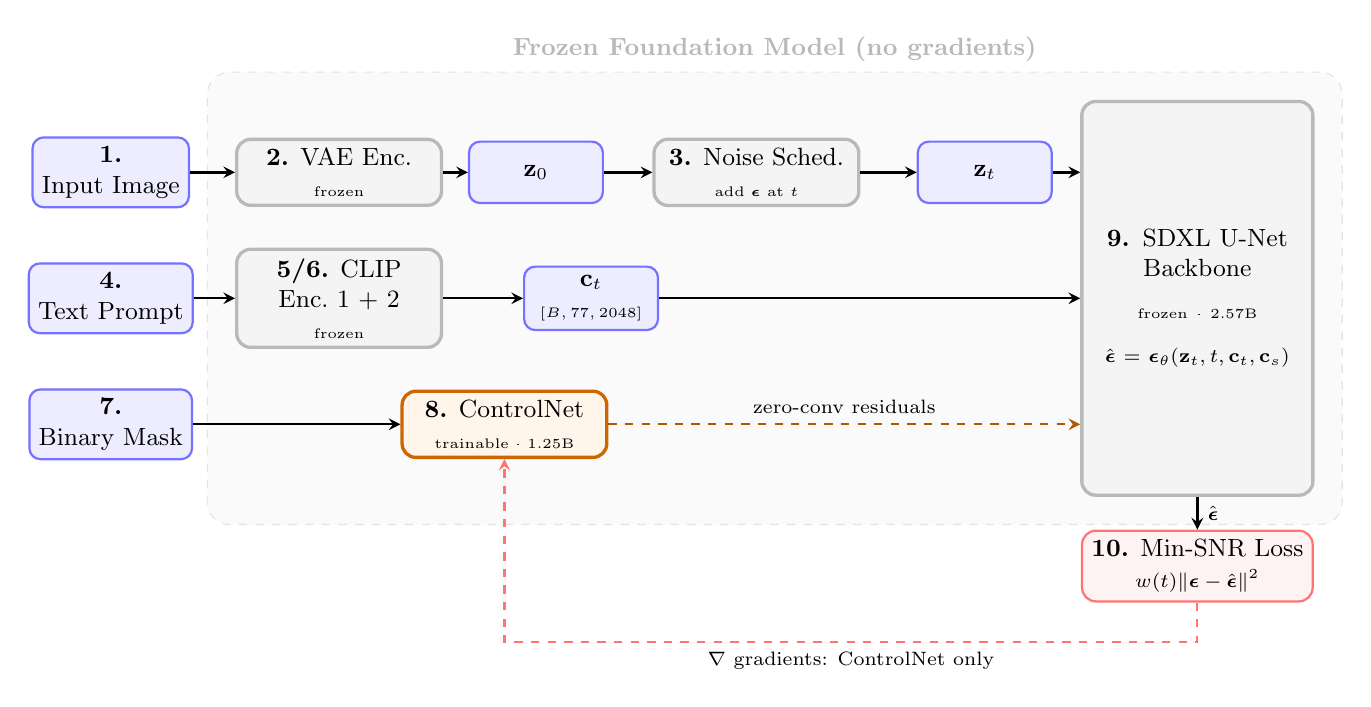
\begin{tikzpicture}[>=stealth, node distance=0.55cm and 1.0cm,
  data/.style={rectangle, rounded corners=4pt,
               minimum width=1.7cm, minimum height=0.78cm,
               align=center, draw=blue!55, fill=blue!7, thick, font=\small},
  frozen/.style={rectangle, rounded corners=5pt,
                 minimum width=2.6cm, minimum height=0.78cm,
                 align=center, draw=gray!55, fill=gray!9, very thick, font=\small},
  trainable/.style={rectangle, rounded corners=5pt,
                    minimum width=2.6cm, minimum height=0.78cm,
                    align=center, draw=orange!80!black, fill=orange!8,
                    very thick, font=\small},
  lossbox/.style={rectangle, rounded corners=5pt,
                  minimum width=2.6cm, minimum height=0.78cm,
                  align=center, draw=red!55, fill=red!5, thick, font=\small},
  arr/.style={->, thick, line width=0.85pt},
  darr/.style={->, thick, dashed, line width=0.85pt, draw=orange!70!black},
  barr/.style={->, thick, dashed, line width=0.8pt, draw=red!55},
]

%% ── ROW 1 (y=1.6):  Image ──────────────────────────────────────────
\node[data]   (img)   at (0.0,  1.6) {\textbf{1.}\\Input Image};
\node[frozen] (vae)   at (2.9,  1.6) {\textbf{2.} VAE Enc.\\{\tiny frozen}};
\node[data]   (z0)    at (5.4,  1.6) {$\mathbf{z}_0$};
\node[frozen] (sched) at (8.2,  1.6) {\textbf{3.} Noise Sched.\\{\tiny add $\boldsymbol{\epsilon}$ at $t$}};
\node[data]   (zt)    at (11.1, 1.6) {$\mathbf{z}_t$};

%% ── ROW 2 (y=0): Text ──────────────────────────────────────────────
\node[data]   (prom)  at (0.0,  0.0) {\textbf{4.}\\Text Prompt};
\node[frozen] (clip)  at (2.9,  0.0) {\textbf{5/6.} CLIP\\Enc.\ 1 + 2\\{\tiny frozen}};
\node[data]   (ct)    at (6.1,  0.0) {$\mathbf{c}_t$\\{\tiny $[B,77,2048]$}};

%% ── ROW 3 (y=-1.6): Mask ───────────────────────────────────────────
\node[data]      (mask) at (0.0, -1.6) {\textbf{7.}\\Binary Mask};
\node[trainable] (cn)   at (5.0, -1.6) {\textbf{8.} ControlNet\\{\tiny trainable · 1.25B}};

%% ── U-Net ───────────────────────────────────────────────────────────
\node[frozen,
      minimum height=5.0cm, minimum width=2.9cm, text width=2.7cm]
     (unet) at (13.8, 0.0)
     {\textbf{9.} SDXL U-Net\\Backbone\\[4pt]{\tiny frozen · 2.57B}\\[5pt]
      {\scriptsize $\hat{\boldsymbol{\epsilon}}=\boldsymbol{\epsilon}_\theta(\mathbf{z}_t,t,\mathbf{c}_t,\mathbf{c}_s)$}};

%% ── Loss ────────────────────────────────────────────────────────────
\node[lossbox] (loss) at (13.8, -3.4)
     {\textbf{10.} Min-SNR Loss\\{\scriptsize $w(t)\|\boldsymbol{\epsilon}-\hat{\boldsymbol{\epsilon}}\|^2$}};

%% ── Row 1 arrows ────────────────────────────────────────────────────
\draw[arr] (img)   -- (vae);
\draw[arr] (vae)   -- (z0);
\draw[arr] (z0)    -- (sched);
\draw[arr] (sched) -- (zt);
\draw[arr] (zt.east) -- (unet.west |- zt.east);

%% ── Row 2 arrows ────────────────────────────────────────────────────
\draw[arr] (prom)  -- (clip);
\draw[arr] (clip)  -- (ct);
\draw[arr] (ct.east) -- (unet.west |- ct.east);

%% ── Row 3 arrows ────────────────────────────────────────────────────
\draw[arr]  (mask.east) -- (cn.west);
\draw[darr] (cn.east) --
    node[above, midway, font=\scriptsize, text=black]{zero-conv residuals}
    (unet.west |- cn.east);

%% ── U-Net → Loss ─────────────────────────────────────────────────────
\draw[arr] (unet.south) --
    node[right, font=\scriptsize]{$\hat{\boldsymbol{\epsilon}}$}
    (loss.north);

%% ── Backprop loop ───────────────────────────────────────────────────
\coordinate (bp0) at ($(loss.south)+(0,-0.5)$);
\coordinate (bp1) at (cn.south |- bp0);
\draw[barr]
    (loss.south) -- (bp0)
    -- node[below, font=\scriptsize, text=black]{$\nabla$ gradients: ControlNet only}
    (bp1) -- (cn.south);

%% ── Background: frozen zone ─────────────────────────────────────────
\begin{scope}[on background layer]
  \node[fill=gray!4, draw=gray!22, rounded corners=8pt, dashed,
        fit=(vae)(sched)(clip)(unet), inner sep=10pt,
        label={[font=\small\bfseries, gray!55]above:Frozen Foundation Model (no gradients)}] {};
\end{scope}

\end{tikzpicture}
\end{document}
